\section{Kết quả}
Kết quả của đồ án được thể hiện qua các hình ảnh sau đây. Kích thước ảnh gốc là 512 x 512 pixel.

\subsection{Ảnh gốc}
\begin{figure}[H]
	\centering
	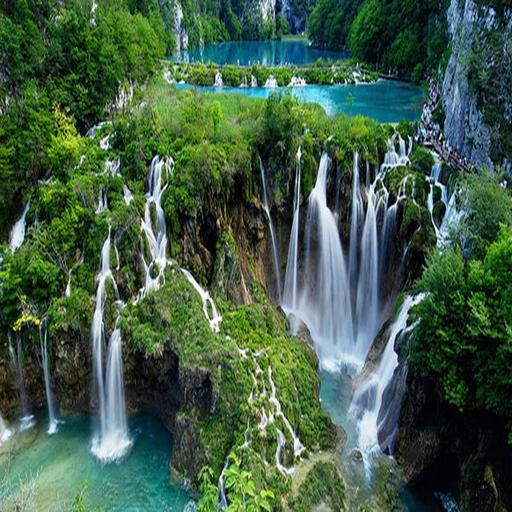
\includegraphics[width=0.5\textwidth]{images/512.jpg}
	\caption{Ảnh gốc}
	\label{fig:original}
\end{figure}

\subsection{Thay đổi độ sáng}
\begin{figure}[H]
	\centering
	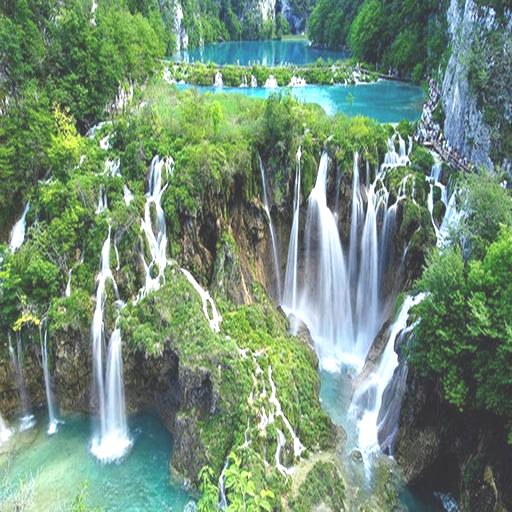
\includegraphics[width=0.5\textwidth]{images/res/512_bright_asc.png}
	\caption{Ảnh tăng sáng nếu nhập vào số dương (50) }
	\label{fig:bright}
\end{figure}

\begin{figure}[H]
	\centering
	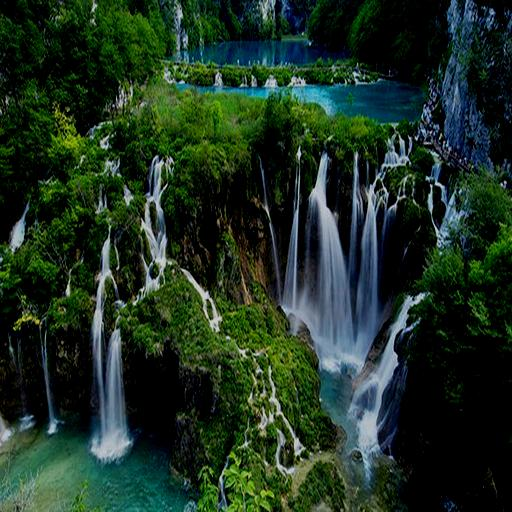
\includegraphics[width=0.5\textwidth]{images/res/512_bright_desc.jpg}
	\caption{Ảnh giảm sáng nếu nhập vào số âm (-50)}
	\label{fig:dark}
\end{figure}

\subsection{Thay đổi độ tương phản}
\begin{figure}[H]
	\centering
	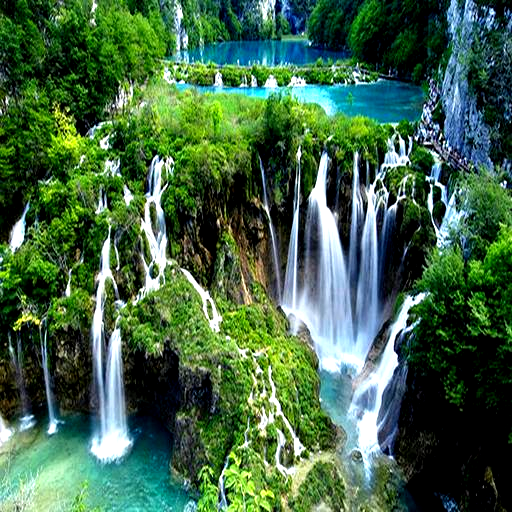
\includegraphics[width=0.5\textwidth]{images/res/512_contrast_asc.png}
	\caption{Ảnh tăng độ tương phản nếu nhập vào số lớn hơn 1 (1.5)}
	\label{fig:contrast_up}
\end{figure}

\begin{figure}[H]
	\centering
	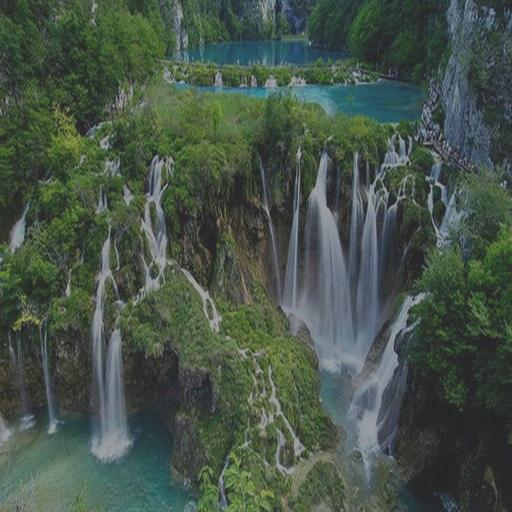
\includegraphics[width=0.5\textwidth]{images/res/512_contrast_desc.jpg}
	\caption{Ảnh giảm độ tương phản nếu nhập vào số nhỏ hơn 1 (0.5)}
	\label{fig:contrast_down}
\end{figure}

\subsection{Ảnh lật ngang}
\begin{figure}[H]
	\centering
	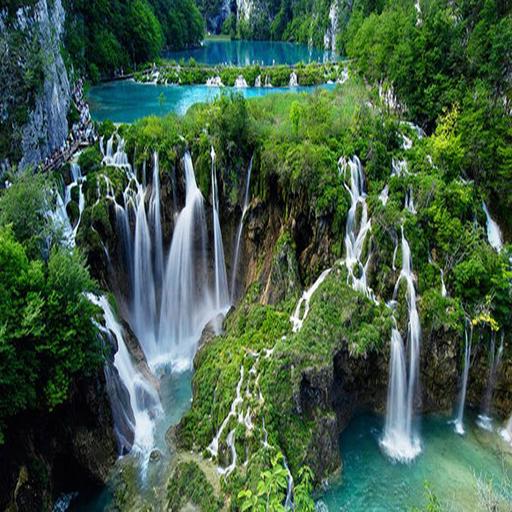
\includegraphics[width=0.5\textwidth]{images/res/512_flip_horizontal.png}
	\caption{Ảnh lật ngang}
	\label{fig:flip_horizontal}
\end{figure}

\subsection{Ảnh lật dọc}
\begin{figure}[H]
	\centering
	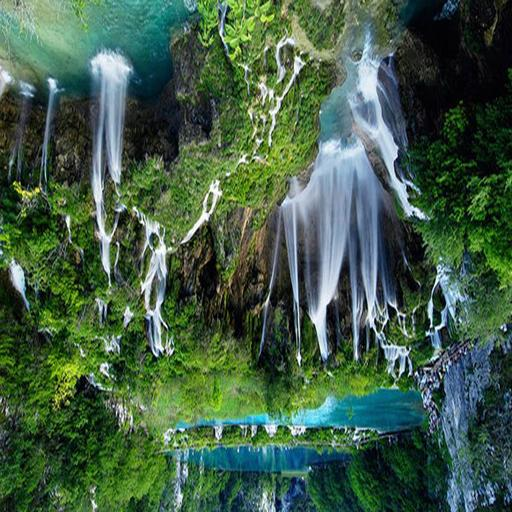
\includegraphics[width=0.5\textwidth]{images/res/512_flip_vertical.png}
	\caption{Ảnh lật dọc}
	\label{fig:flip_vertical}
\end{figure}

\subsection{Chuyển đổi sang ảnh xám}
\begin{figure}[H]
	\centering
	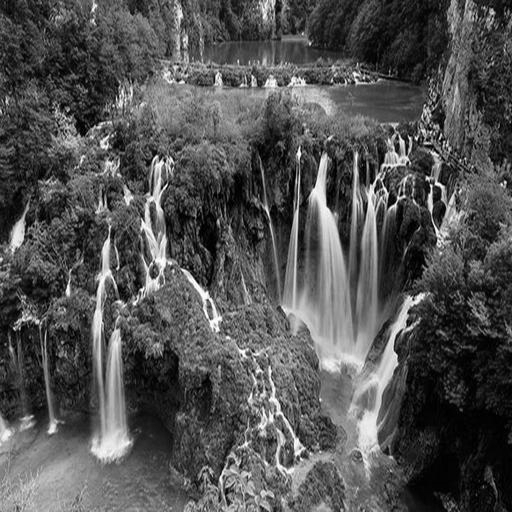
\includegraphics[width=0.5\textwidth]{images/res/512_grayscale.png}
	\caption{Ảnh chuyển sang ảnh xám}
	\label{fig:gray}
\end{figure}

\subsection{Chuyển đổi sang ảnh sepia}
\begin{figure}[H]
	\centering
	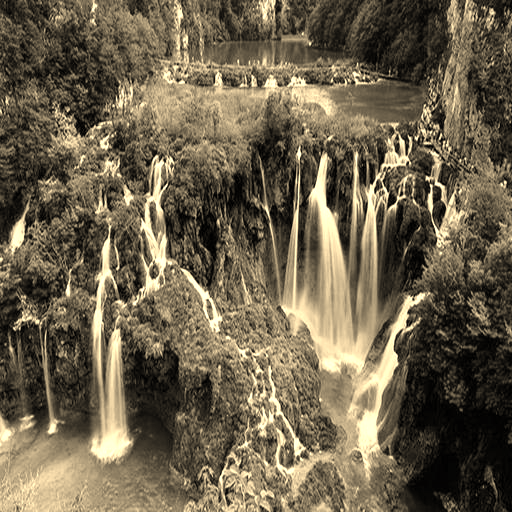
\includegraphics[width=0.5\textwidth]{images/res/512_sepia.png}
	\caption{Ảnh chuyển sang ảnh sepia}
	\label{fig:sepia}
\end{figure}

\subsection{Làm mờ ảnh}
\begin{figure}[H]
	\centering
	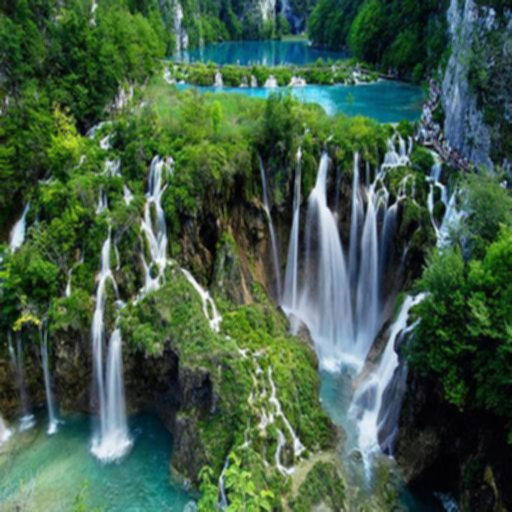
\includegraphics[width=0.5\textwidth]{images/res/512_blur3.png}
	\caption{Ảnh làm mờ với kernel 3x3}
	\label{fig:blur}
\end{figure}

\begin{figure}[H]
	\centering
	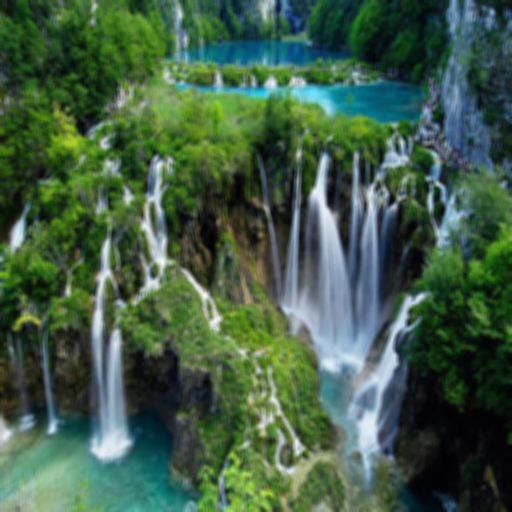
\includegraphics[width=0.5\textwidth]{images/res/512_blur5.png}
	\caption{Ảnh làm mờ với kernel 5x5}
	\label{fig:blur}
\end{figure}

\subsection{Làm sắt nét ảnh}
\begin{figure}[H]
	\centering
	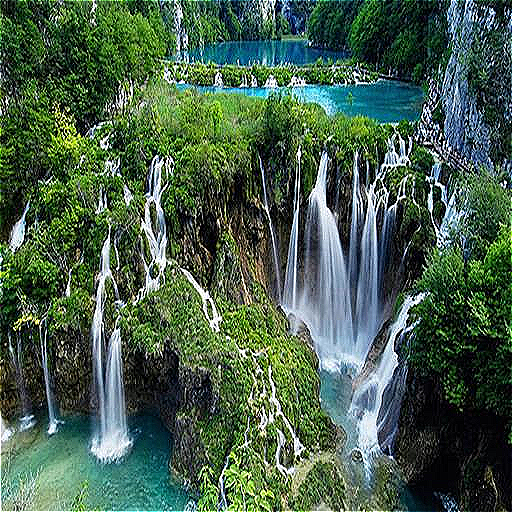
\includegraphics[width=0.5\textwidth]{images/res/512_sharpened.png}
	\caption{Ảnh làm sắt nét với kernel 3x3}
	\label{fig:sharpen}
\end{figure}

\subsection{Cắt ảnh theo kích thước trung tâm}
\begin{figure}[H]
	\centering
	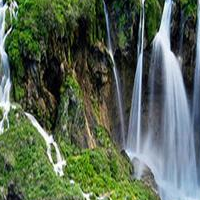
\includegraphics[width=0.5\textwidth]{images/res/512_crop_center.png}
	\caption{Ảnh cắt theo kích thước trung tâm (200 x 200 pixel)}
	\label{fig:crop_center}
\end{figure}

\subsection{Cắt ảnh theo khung hình tròn}
\begin{figure}[H]
	\centering
	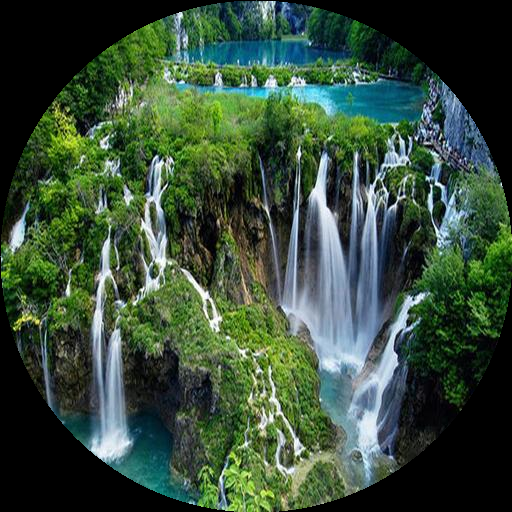
\includegraphics[width=0.5\textwidth]{images/res/512_crop_circle.png}
	\caption{Ảnh cắt theo khung hình tròn}
	\label{fig:crop_circle}
\end{figure}

\subsection{Cắt ảnh theo khung 2 hình elip chéo nhau}
\begin{figure}[H]
	\centering
	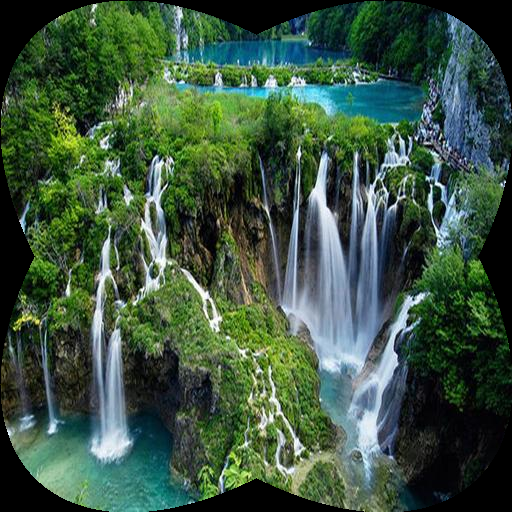
\includegraphics[width=0.5\textwidth]{images/res/512_crop_ellipse.png}
	\caption{Ảnh cắt theo khung 2 hình elip chéo nhau (ratio = 0.75)}
	\label{fig:crop_ellipse}
\end{figure}


\subsection{Thời gian chạy}
\begin{table}[H]
	\centering
	\caption{Thời gian chạy của các thuật toán xử lý ảnh}
	\label{tab:execution_time}
	\begin{tabular}{|l|c|}
		\hline
		\textbf{Thuật toán}                      & \textbf{Thời gian chạy (giây)} \\ \hline
		Thay đổi độ sáng                         & < 1                            \\ \hline
		Thay đổi độ tương phản                   & < 1                            \\ \hline
		Lật ảnh ngang                            & < 1                            \\ \hline
		Lật ảnh dọc                              & < 1                            \\ \hline
		Chuyển đổi sang ảnh xám                  & < 1                            \\ \hline
		Chuyển đổi sang ảnh sepia                & < 1                            \\ \hline
		Làm mờ ảnh (kernel 3x3)                  & 5.32                           \\ \hline
		Làm mờ ảnh (kernel 5x5)                  & 8.05                           \\ \hline
		Làm sắt nét ảnh                          & < 1                            \\ \hline
		Cắt ảnh theo kích thước trung tâm        & < 1                            \\ \hline
		Cắt ảnh theo khung hình tròn             & < 1                            \\ \hline
		Cắt ảnh theo khung 2 hình elip chéo nhau & < 1                            \\ \hline
	\end{tabular}
\end{table}